\chapter{Problems in Audio Scene Analysis}\label{ch:application}

\newthought{Synopsis} \synopsisChApplication

\mynewline
Following the structure of the previous part, this chapter gathers the common knowledge shared across the following chapters.
In particular, it present some audio scene analysis problems that will be later discussed in their echo-aware extention.
The literature for each of them is reviewed, but since it is vast and spans diverse decades of scientific research, we do not aim to cover it entirely.
Moreover, since the following chapters are dedicated to each of these problems under the echo-aware perspective, the echo-aware literature is not considered here.

\mynewline
The material presented here results from the personal elaboration of concepts and references available in the literature.
Furthermore, some definitions are digested from classical textbooks already used for this thesis, such as~\citeonly{vincent2018audio}, and audio signal processing lecture notes.

\section{Audio Scene Analysis Problems}\label{sec:application:scenario}
As mentioned in the first chapter, the audio scene analysis aims to parcel all the relevant information in the indoor audio scene.
Different types of information are estimated or inferred by different audio signal processing algorithms solving specific problems.
Despite their diversity, most of these problems can be defined on a common model for the microphone observations.

\subsection{Common scenario and common model}
Let there be a meeting room with well-defined geometry.
In it, $\numSrcs$ sound sources are located at determined positions, such as some speakers chatting while standing in the room.
As it is a indoor scenario, all the elements of reverberation (in particular echoes) are presents.
Diffuse background noise is present as well, for instance, due to the air conditioner or car traffic outside.
This whole audio scene is recorded by a device featuring a microphone array of $\numMics$ sensors.
Furthermore we assume a static far field scenario and we model each $\idxSrc$ sources and $\idxMic$ microphone as well-defined points with coordinate $\positionSource$ and $\positionMicrophone$, respectively.
This is a reasonable assumption in the context of table-top devices, such as smart home devices.

\begin{figure}[]
    \begin{sidecaption}[Audio Scene]{%
        Cartoon of a audio scene.
    }[fig:estimation:activepassive]
    \centering
    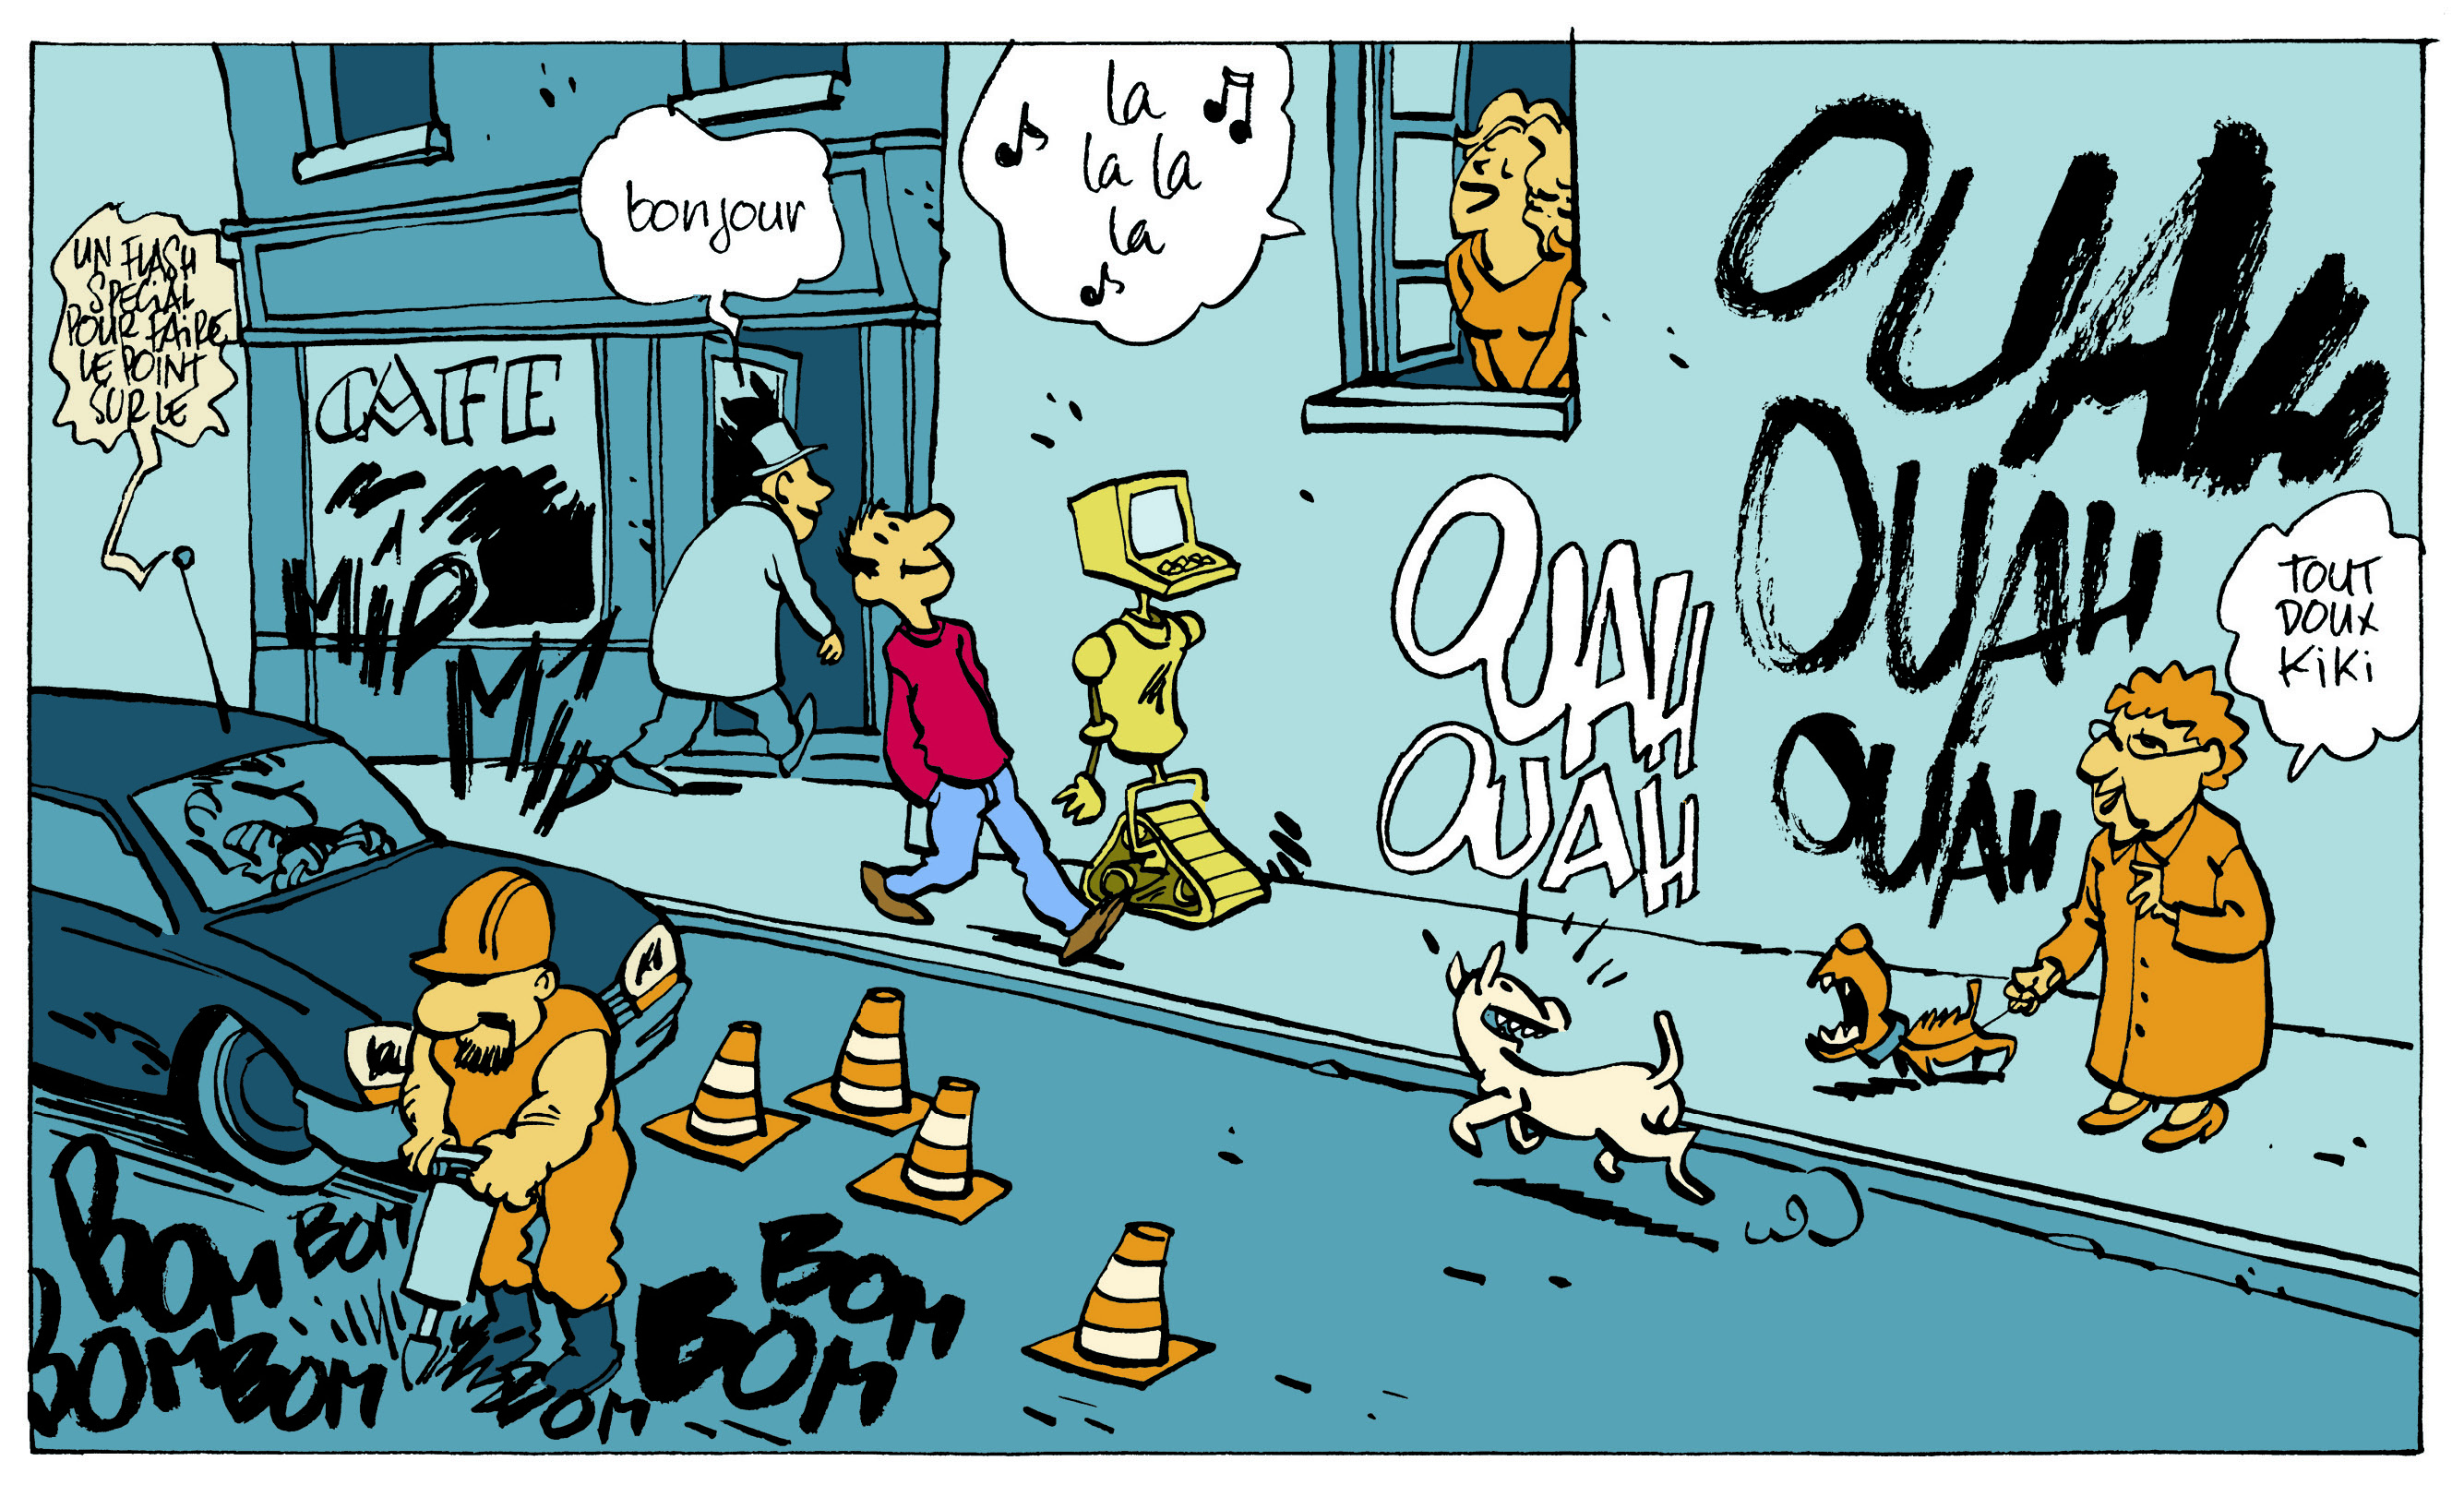
\includegraphics[width=\linewidth]{application/audio_scene.jpg}
    \end{sidecaption}
\end{figure}

Recalling the (discrete) time-domain signal model~\cref{ch:processing:blabal} already discussed the relative chapter, the signal recorded at the $\idxMic$-th microphones reads
\begin{equation}
    \label{eq:application:stft}
    \mic_\idxMic[n] = \sum_{\idxSrc = 1}^{\numSrcs}
        \kparen{\flt_{\idxMicSrc}( \positionMicrophone_{\idxMic}  | \positionSource_{\idxSrc}) \convDis \src_{\idxSrc}} [n] + \nse_\idxMic[n]
    .
\end{equation}
Note that the filter $\flt_{\idxMicSrc}(\positionMicrophone_{\idxMic} | \positionSource_{\idxSrc})$ denotes the \RIR/ where we intentionally highlight the dependencies on geometry,
namely, accounting for the whole sound propagation for the source position $\positionSource_{\idxSrc}$ to the microphone position $\positionMicrophone_{\idxMic}$.
In fact, as discussed throughout~\cref{ch:acoustics,ch:processing}, we can decouple the information of indoor microphone natural recordings into two orthogonal contributions:
the \RIRs/ (thus the mixing matrix) accounting for only the sound propagation, and the source signals that depend only on the sound content.

\newcommand{\setMicSignals}{\ensuremath{\set{\mic_{\idxMic}}_\idxMic}}
\newcommand{\setSrcSignals}{\ensuremath{\set{\src_{\idxSrc}}_\idxSrc}}
\newcommand{\setSrcPositions}{\ensuremath{\set{\positionSource_{\idxSrc}}_\idxSrc}}
\newcommand{\setFltSignals}{\ensuremath{\set{\flt_{\idxMicSrc}(\positionMicrophone_{\idxMic} | \positionSource_{\idxSrc})}_{\idxMicSrc}}}


\subsection{Problems formulation}
The Audio Scene Analysis Problems presented already in the introductory chapter (See~\cref{sec:intro:scene}) can be now extended and rewritten in terms of the above notation.
Furthermore, we will consider here the only ones directly addressed in this thesis, namely, room impulse response estimation, audio source separation, spatial filtering, sound source localization, and room geometry estimation.

\begin{table}[!h]

    \begin{fullwidth}
    \centering
    \small
    \renewcommand{\arraystretch}{1.3}

    \begin{tabular*}{\linewidth}{@{\extracolsep{\fill}}lllll@{}}
    \toprule
    Audio scene analysis problems & \textit{from the mixtures $\setMicSignals$, can we estimate...}  & Chapter\\
    \midrule

    Audio Source Separation     & \begin{tabular}[c]{@{}l@{}}the source signals $\setSrcSignals$ and\\ \hspace{1em} the filters $\setFltSignals$?\end{tabular}   & \cref{ch:separake}\\

    Spatial filtering           & \begin{tabular}[c]{@{}l@{}}the source signals $\setSrcSignals$,\\ \hspace{1em} knowing the filters $\setFltSignals$?\end{tabular} & \cref{ch:decharateapp}~\cref{sec:dechorateapp:se}\\

    Sound Source Localization   & the source positions $\setSrcPositions$?                              & \cref{ch:mirage}\\

    Room Geometry Estimation    & the shape of the room?                                                & \cref{ch:decharateapp}~\cref{sec:dechorateapp:rooge}\\
    \bottomrule
\end{tabular*}


% Channel (or \RIR/) Estimation            & the filters $\setFltSignals$ ?                            & \cref{pt:estimation}\\

% Acoustic Echo Retrieval     & the early echoes' timings and gain accounted in $\setFltSignals$ ?     & \cref{pt:estimation}\\

% \RIR/ measurement           & the filters $\setFltSignals$, knowing $\setSrcSignals$ ?               & \cref{ch:dechorate}\\
% Speech Enhancement          & the signal of the $\idxSrc$-th target source $\src_{\idxSrc}$?        & \cref{ch:decharateapp}\\

    % \hline

    \caption{List of audio scene analysis problems considered in this thesis accompanied with their mathematical description.}
    \label{tab:processing:problems}

    \end{fullwidth}

\end{table}

\mynewline
As introduced in~\cref{sec:estimation:problem}, depending on the application, these problems can be said either \textit{informed} or \textit{blind} and the related scenario \textit{active} or \textit{passive}.
These two dichotomies emphasize the amount of prior knowledge available for solving them.
As opposed to the active scenario, where the source signal is known, transmitted, and available, the passive one considers only the microphone measurements.
For instance, when addressing the active echo estimation problem or \RIR/ measurement, the exact time of emission of the source signal is known, as well as the source signal itself.
\\The second dichotomy refers to the possibility of exploiting prior knowledge to facilitate the solution of the problem.
This information may derive from annotations, meta-data that accompany the application.
In the community of audio source separation, the following definitions were proposed in~\citeonly{vincent2014blind}:
as opposed to informed problems, for solving the blind ones, absolutely no information is given about the source signal or the mixing process.
In between, there are \textit{semi-blind} and \textit{strongly guided} problems:
For the formers, general information is available, such as on the nature of the source signal (speech, music, environmental sounds),
microphone position, recording scenario (indoor, outdoor, professional music) \etc/.
For the latters, specific information such as about the mixing process, the identity of the speakers can be used.

\mynewline
In this part of the thesis, we will consider echo-aware applications where the echoes properties build our prior knowledge on the problem.
Therefore, the addressed problems are necessarily strongly-guided.
In general, and unless specified, this is the only knowledge we assume to have.
Based on this, we will now review some classical methods for solving the above problems.


\section{Literature overview}\label{sec:application:sota}
Here we present the general overview of the literature related to the problems considered in this thesis: multichannel audio source separation, and spatial filtering, and sound source localization.
We will limit the discussion to the most relevant techniques adopted nowadays and the acoustic propagation modeling.
Later, dedicated sections on echo-aware method to address these problems will be provided in each of the following chapters .
Since \RooGE/ is manly based on echo estimation and labeling, the its discussion is reported in~\cref{subsec:estimation:active_rir, subsec:dechorateapp:rooge}.

\subsection{on Multichannel Sound Source Separation}
Multichannel audio source separation refers to the process of extracting acoustic signals from multichannel mixtures featuring targets, interfering and noisy sounds.
In pyschoacoustics, this problem is known as \textit{the cocktail party problem}~\citeonly{cherry1953cocktail}, referring to the human ability to focus on a particular stimulus in the audio scene.
In the literature this problem is mainly investigated for two types of data: music and speech signal recordings~\citeonly{[Vincent et al., 2012]}.
This focus of this thesis is on speech source separation nevertheless share
This is of interest for several audio applications, such as: speech enhancement [Mohammadiha et al., 2013], crosstalk cancellation [Akeroyd et al., 2007], hearing aids [Healy et al., 2013], and automatic speech recognition [Li et al., 2014]

Echoes have been used previously to enhance various audio processing tasks.

[Remaggi thesis]
During the last twenty years, speech separation has gained quite of attention. Some of the proposed methods achieved source separation exploiting the availability of a single microphone [Jang and Lee, 2003, Radfar and Dansereau, 2007, Schmidt and Olsson, 2006]. However, they were limited by the amount of information utilised. Therefore, other methods attempted the separation process by employing multichannel microphone arrays. These methods are classically categorised into three main groups, depending on the type of approach undertaken [Vincent et al., 2012]: the beamformers [Araki et al., 2003, Coleman et al., 2015a, VanVeen and Buckley, 1988]; the independent component analysis (ICA) based [Bell and Sejnowski, 1995, Cardoso, 1998, Makino et al., 2007]; the time-frequency (TF) mask based [Alinaghi et al., 2014, Deleforge et al., 2015, Mandel et al., 2010, Sawada et al., 2011, Yilmaz and Rickard, 2004]. A visualisation of these three


I think you need to reorient this section to include other, more state-of-the art methods in multichannel source separation, and provide a justification why multichannel NMF (a 10 years old approach) is used here.
I think a good point to make is that the specific goal of this work is to show the benefit of adding a multichannel early echo model on top of a coarse source spectral model (provided here by NMF).
This could not be done using end-to-end multichannel deep-learning based methods (you should nevertheless cite some of them).
The proposed approach could also be easily applied to the work of [Nugraha et al. 2016] which builds on EM-NMF.
But we chose NMF for its simplicity, its small training-data requirements, and its ability to include speaker-specific dictionaries [which Nugraha et al. 2016 can't do].
You should also at least include references to other multichannel NMF methods, i.e., the ones proposed by Sawada et al.

According to the definition given in~\cref{ch:processing}, audio source separation algorithms can be grouped according to how they model with sound propagation in the mixing process:
\begin{itemize}
    \item those that ignore it \citeonly{le2015deep} (instantaneous mixing process);
    \item those that assume a single anechoic path \citeonly{rickard2007duet, nesta2012convolutive} (anechoic mixing process);
    \item those that model the \RTFs/ entirely \citeonly{ozerov2010multichannel, duong2010under, nugraha2016multichannel, li2019expectation} (convolutive mixing process);
    \item and those that attempt to separately estimate the contribution of the early echoes and the contribution of the late tail \citeonly{leglaive2015multichannel}.
\end{itemize}

\subsection{on Spatial Filtering}
Beamformers combines the channels of multiple microphones in order to achieve spatial selectivity, suppressing noise, interferences and reverberation~\citeonly{VanTrees2004Optimum}.

\newthought{Current Challenges}

\subsection{on Sound Source Localization}
\SSLdef/ consists in determining the position of sources from microphone recordings in the 3D space.
The sources' and microphones' positions in the room are encoded the \RIRs/.
Therefore, assuming the uniqueness of the mapping between locations to a \RIR/, it is theoretically possible to retrieve the absolute position of microphones and sources.
However, as deeply discussed in~\cref{ch:estimation} and shown in the work~\citeonly{crocco2017uncalibrated}, this is already a very challenging task, which may involves the solution of many several sub-problems.
Therefore, it is more common to relax the \SSL/ problem as follows:
First, rather the sources 3D coordinates, most of existing methods aim at estimating the 2-dimensional \DOAdef/, namely, \textit{azimuth} and \textit{elevation} angles with respect to a reference point in the microphone array\sidenote{typically the baricenter.}.
Second, they assume far-field scenarios.
The main reason for adopting such simplifications is two-fold:
on one side, estimating the distance is know to be a much more challenging task, than estimating the \DOAs/~\citeonly{vesa2009binaural}.
on the other side, many far-field speech enhancement methods require only the sources' \DOAs/ as only knowledge.

\mynewline
Despite these approximation, the \SSL/ problem still challenges today's computational methods, in particular in the presence of reverberation or interfering sources (see \cite{rascon2017localization} and \cite{Argentieri2015} for a review).


In We can iden two components.
First, extracting features from audio data that are as independent as possible from the source's content while preserving spatial information.
Second, mapping these features to the source position.
Two lines of research have been investigated to obtain such mappings: physics-based and learning-based approaches.

\newthought{Physics-based approaches} rely on a simplified sound propagation model \cite{rascon2017localization,Knapp1976,DiBiase2001,Lebarbenchon2018}.
The free-field model is by far the most widely used one and assumes
a single direct sound path from the source to each microphone.
When the source is placed far enough, this yields a closed-form mapping from the
sound's time-difference-of-arrival (TDOA) in a microphone pair and the source's azimuth angle in this pair.
If multiple microphone pairs are available and form a non-linear array,
their TDOAs can be aggregated to obtain 2D directions of arrival \cite{DiBiase2001}.
These methods strongly suffer in environments where the free-field assumption is violated,
\textit{e.g.}, in the presence of strong acoustic echoes and reverberation \cite{Scheuing2006}.

\newthought{Learning-based approaches} use an annotated training dataset to implicitly
learn a mapping from audio features to source positions
\cite{deleforge2015acoustic, Vesperini2016, Adavanne2017,  Perotin2018, gaultier2017vast}.
Such data can be obtained from real recordings \cite{deleforge2015acoustic} or
using physics-based simulators \cite{Vesperini2016, Adavanne2017,  Perotin2018, gaultier2017vast}.
These methods were showed to overcome some limitations of the free-field model,
but are usually trained for specific microphone arrays and fail whenever test conditions strongly mismatch training conditions.

\newthought{Current Challenges}

% \subsection{An acoustic perspective}\cite{subsec:application:sota_propagation}
% Bibliography with respect to sound propagation
% \begin{itemize}
%     \item Ignored
%     \item Anechoic Phat
%     \item Fully modeled
%     \item Early echoes
% \end{itemize}


% \subsection{An algorithmic perspective}\cite{subsec:application:sota_estimation}
% Bibliography with respect to learning and knowledge approaches


\section{Conclusion}\label{sec:application:conclusion}
In this chapter we draw a line

Based on this idea, so-called \textit{echo-aware} methods have been introduced few decades ago, where matched filters (or rake receivers) are used to constructively sum the sound reflections \citeonly{Jan1995matched, Affes1997signal} and build beamformers achieving much better sound qualities \citeonly{gannot2001signal}.
This methods have recently regained interested as manifested by the European project SCENIC~\citeonly{Annibale2011scenic} and the UK research \href{http://www.s3a-spatialaudio.org/}{S$^3$A project}.
They show that knowing the properties of a few early echoes can boosts performances of typical indoor audio inverse problems such as speech enhancement (SE) \citeonly{Dockmanic2015raking, Kowalczyk2019raking}, sound source localization \citeonly{ribeiro2010turning, DiCarlo2019mirage}, and separation \citeonly{scheibler2017separake, leglaive2016multichannel}.
Another fervent area of research spanning transversely the audio and acoustic signal processing fields is estimating the room geometry blindly from acoustic signals.
As presented by Crocco \textit{et al.} in \citeonly{crocco2017uncalibrated}, the end-to-end room geometry estimation (RooGE) involves many subsequent subtasks:
RIR estimation, peak picking, microphones calibration, echo labeling, reflectors estimation. Acoustic echo retrieval (AER) is common to many of these topics. It consists in estimating the properties of echoes such as their TOAs and energies. The former problem is referred to as TOA estimation, or time-delay estimation when the direct-path is taken as reference. Furthermore, as interesting applications, these methods have been recently used in active scenarios, namely knowing the transmitted signals, using unmanned aerial vehicle (UAV, a.k.a. drones) \citeonly{jensen2019method, Boutin2020drone} and mobile-phones \citeonly{Shih2019phone}.





%% models %%
% \newthoughtpar{end2end \vs/ 2step}
% end2end: from data to (feature to) target
% \\2-step: (from data to features) + features to target

% \newthoughtpar{Knowledge-based \vs/ Learning-based}
% \begin{itemize}
%     \item Bottom-up vs Top-down information processing
%     \item Knowledge-based: specialized signal processing and mathematical algorithms informed by knowledge;
%     \item Learning-based: machine learning usually trained in supervised fashion.
% \end{itemize}
